%卒業論文用テンプレート
\documentstyle[graphicx]{jronbun}

%諸定義
\newenvironment{indention}[1]{\par
\addtolength{\leftskip}{#1}
\begingroup}{\endgroup\par}

%論文名
\title{センシング技術を用いたモビリティショッピング端末の開発}
%教官名
\kyoukan{高橋寛教授}
\second{王森レイ講師}
%名前
\author{真鍋 樹}
%提出日
\date{令和2年~月~日提出}
%講座名
\kouza{\gt 愛媛大学工学部情報工学科情報システム工学講座}

\begin{document}
%タイトル生成
\maketitle
%目次生成
\pagenumbering{roman}
\tableofcontents
\cleardoublepage
\pagenumbering{arabic}

%--ここから本文--
%第1章 まえがき
\chapter{まえがき}
%まえがき
現在の日本では少子高齢化の進行による人的資源が減少している。総務省の平成28年度の人口調査では2030年には1億1662万人に減少し、2050年には人口が1億人下回ると見込まれる\cite{population}。人的資源の減少という問題は社会全体に関わることである。人手不足問題解消のために、各産業では業務の無人化が急務となっている。

最近、サービス業者にも人手不足の問題が深刻化おり、セルフレジの導入が進んでいる。しかしながら、セルフレジは導入コストが高いという問題がある。セルフレジは、登録機と精算機を合わせて平均で300万を超える\cite{self_register}。セルフレジの導入は、人手不足問題を抱える店舗においてメリットも大きいが負担も大きい。特に小規模な店舗の導入における負担が大きく、既存のセルフレジより安価で導入しやすいシステムが求められている。

これらの問題を解決するために、資金力を持たない店舗でも導入しやすく、安価で人手のかからないシステムの提案と開発を本研究の目的とした。本研究の目的としては、バーコードスキャン技術を利用したスマートモビリティレジシステムを開発することである。

本研究では、商品の識別から決算までのシステム構築をV字開発モデルに従い、グループ(段原丞治、真鍋樹)で研究を行った。
要求定義や設計はUML(Unified Modeling Language)図を用いて定義し、それをもとにシステムの設計と実装を行う。実装では、エッジ処理側とサーバ処理側で担当を分けた。エッジ側のハードウェアはRaspberryPiを使用した。サーバは画像処理をYolo(画像から物体を識別する機械学習ネットワーク)\cite{yolo}やOpenCV(画像処理ライブラリ)\cite{opencv}等を利用して行う。

本論文は、以下のような構成をとる。第2章では、本研究で使用した用語、技術の解説を述べる。第3章では、UML図を用いてシステムの要求定義、設計、検証項目を述べる。第4章では、実装内容と検証結果を示す。第5章では、実装したシステムの評価及び考察を述べる。第6章では、本研究のまとめを示す。

%第2章 準備
\chapter{準備}
%第2章:準備
本章では本文中に使用する用語、実験環境およびシステム概要について述べる

\section{諸定義}

\subsection*{V字モデル}
V字モデルとはシステム開発を要求分析、基本設計、詳細設計、実装に分け上から順にそれぞれに対して検証、テストを行いながら上から順に時間軸に従って行っていく。細かく要素ごとにテストをしていくことで開発の途中で大幅な変更や問題が起きにくくなる利点がある。

\begin{figure}[htbp]
\centering
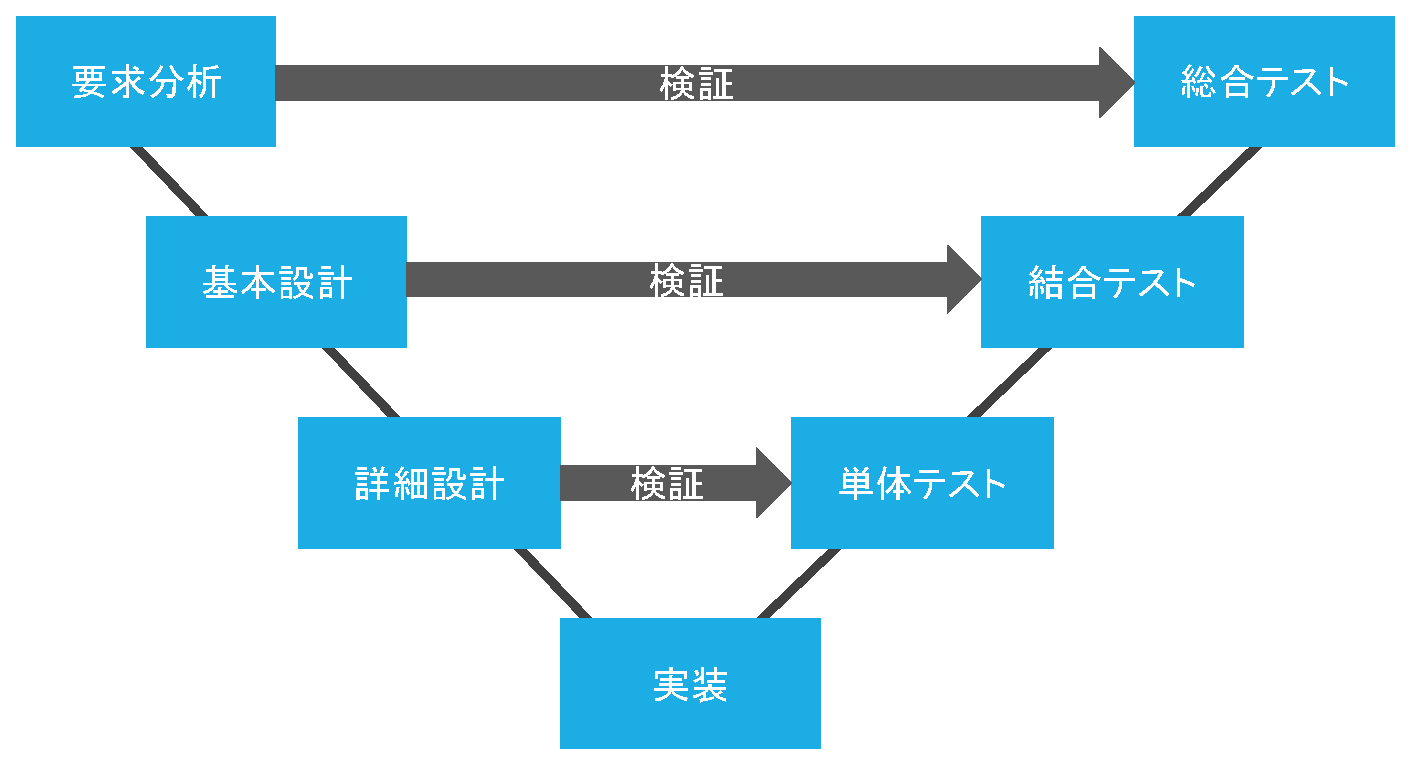
\includegraphics[width=12cm]{./pic/vjimodel.eps}
\caption{V字モデル}
\label{v_model}
\end{figure}

\subsection*{UML(Unifiled Modeling Language)}
UMLとは各開発工程で利用すべき図面の標準化されたモデルである。UMLで一番重視されていることは、単純で分かりやすいという軸と十分実用に使えるだけの強力な表現方法を持つ軸を最適に組み合わせて言語設計をすることである。UMLの構成要素としてユースケース図、クラス図、シーケンス図がある。\cite{uml}

\subsection*{ユースケース図}
システムがどのように機能すべきかという振る舞いとその外部環境を表す。


\subsection*{シーケンス図}
シーケンス図は、オブジェクト間のメッセージのやり取りを時系列順に沿って並べて表現したもの。
ユースケース図を基にしてシーケンス図やクラス図を制作していく。

\subsection*{クラス図}
クラス図はモデルの静的な構造を示す図。クラスが持つ動作や、属性を記述する。より具体的な実装部分に近い記述をしていく。

\subsection*{Yolo(Real-Time Object Detection)}
Yoloはリアルタイムでのオブジェクト識別が可能なネットワークを目的としている。Webカメラでのリアルタイム検出を行うこともできるFPSを誇る。ほかのネットワークとの違いは検出と、識別を同時に行っているため高速性を保てる点である。今回は画像からバーコードの位置を特定するために使用した。\cite{yolo}.


\subsection*{pyzbar}
バーコード画像データを解析して数字を識別するライブラリである。\cite{pyzbar}.

\section{システムの概要}
 システムでは、買い物かごにエッジ処理を担当するRaspberryPiと各種センサを設置する。エッジ側では商品の特定に必要となるデータをセンサ類を用いて取得する。データを取得したらサーバ側に送信し、そこで画像データを処理して商品の特定を行う。システムの流れを以下の図\ref{system_summary}に示す。


\begin{figure}[htbp]
\centering
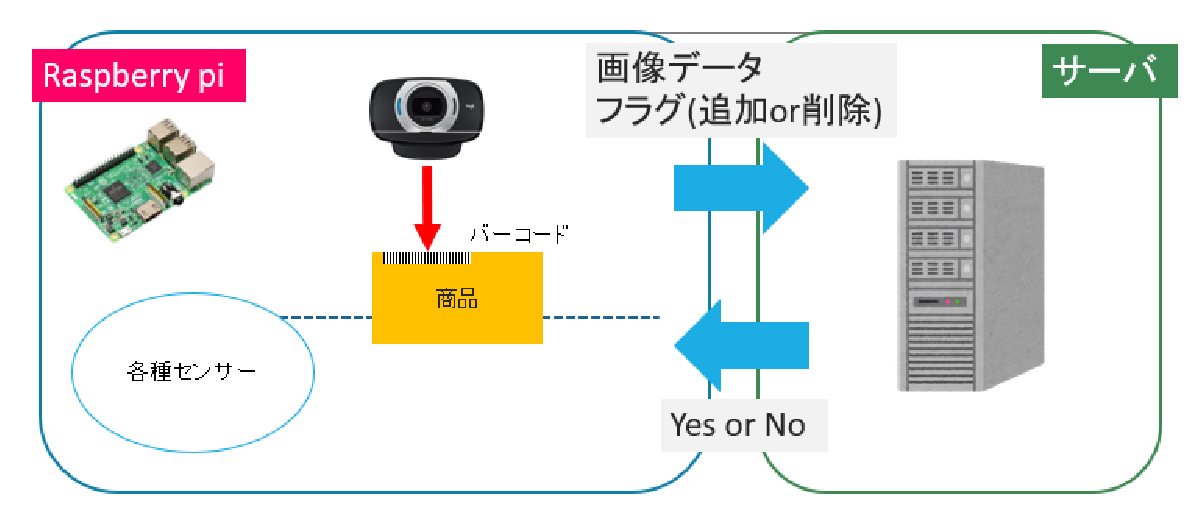
\includegraphics[width=12cm]{./pic/summary.eps}
\caption{システムの流れ}
\label{system_summary}
\end{figure}

左側のRaspberryPi側で商品に関するデータをサーバに送信する。画像のフラグは送信された画像の商品がかごから追加されるものなのか削除されるものなのかを判断するのに使用する。サーバはデータを受け取ったのちバイナリーデータから画像データに戻す。画像からバーコード番号が識別できた場合、追加・削除のフラグに従ってDBを更新する。そしてRaspberryPiに識別が成功したフラグを返信する。


\section{実験環境}
 実験環境で使用したものを以下の表に示す。
\begin{table}[htb]
\begin{center}
\caption{実行環境}
\begin{tabular}{|c|c|c|c|c|} \hline
処理担当 & OS & CPU & RAM & GPU \\ \hline
サーバ側 & Windows10 64bit Pro & Core2Duo & 4GB & GT740 \\ \hline
エッジ側 & RaspberryPi3B+(Rasbian) & 1.2GHz & 1GB & None \\ \hline
\end{tabular}
\label{spec}
	\end{center}
\end{table}




%第3章 
\chapter{スマートモビリティレジシステムの設計}
%第3章
本章ではV字モデルによる要求定義および設計について述べる。本章の構築は以下のとおりである。3.1節ではユースケース図を用いて要求定義を説明する。3.2節では、クラス図を用いて、基本設計及び詳細設計を述べる。


\section{要求定義}
 ユーザがシステムに求める機能や動作を決定する。以下に要求定義をまとめた図\ref{usecase}を載せる。
\ref{usecase}では、ユーザがシステムに対して動作を行った際にどのような振る舞いをするか記載してある。ユーザは通常の買い物のようにカートに商品を出し入れすることができる。このときカート(RaspberryPi)が商品に関するデータを集める。解析システムでは画像から商品の特定やカゴDBへの操作を行う。この解析システムはサーバで動作する。カゴDBではカート内にある商品の管理を行う。ここで管理されている情報が最終的な決済システムで利用される。ユーザはカートを返却すると決済システムが動作し自動で決済システムが動作し顧客の所持金からカート内の商品合計金額がひかれる。

\begin{figure}[htbp]
\centering
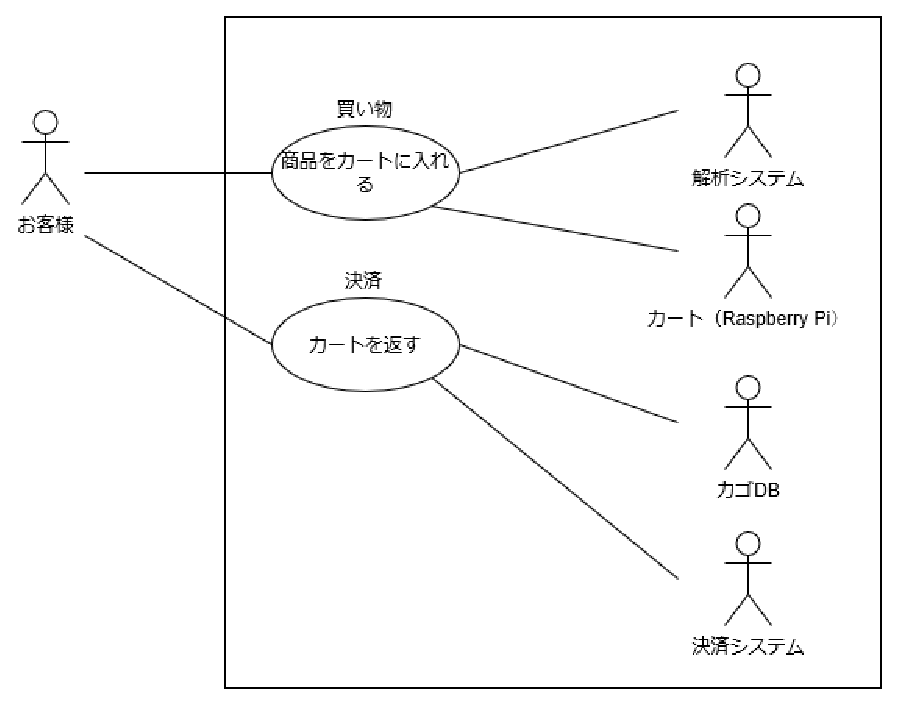
\includegraphics[width=12cm]{./pic/usecase_saishu.eps}
\caption{ユースケース図}
\label{usecase}
\end{figure}
\section{要求定義}
ユーザが商品識別システムに求める機能や動作を以下に述べる。以下に要求定義をまとめた図\ref{usecase}を載せる。赤枠で囲っている部分が筆者が担当した。
\ref{usecase}では、ユーザが商品識別システムに対して動作を行った際に、システムがどのような振る舞いをするか記載した。ユーザは通常の買い物のように、カートに商品を出し入れすることができる。このときカート(RaspberryPi)が商品に関するデータを集める。解析システムでは、商品の特定とカゴDBへの操作を行う。この解析システムはサーバで動作する。カゴDBは、カート内にある商品の管理を行う。ここで管理されている情報が、最終的な決済システムで利用される。ユーザがカートを返却すると、決済システムが動作する。決済システムは、顧客の所持金からカート内の商品合計金額を引く処理を行う。

\begin{figure}[htbp]
\centering
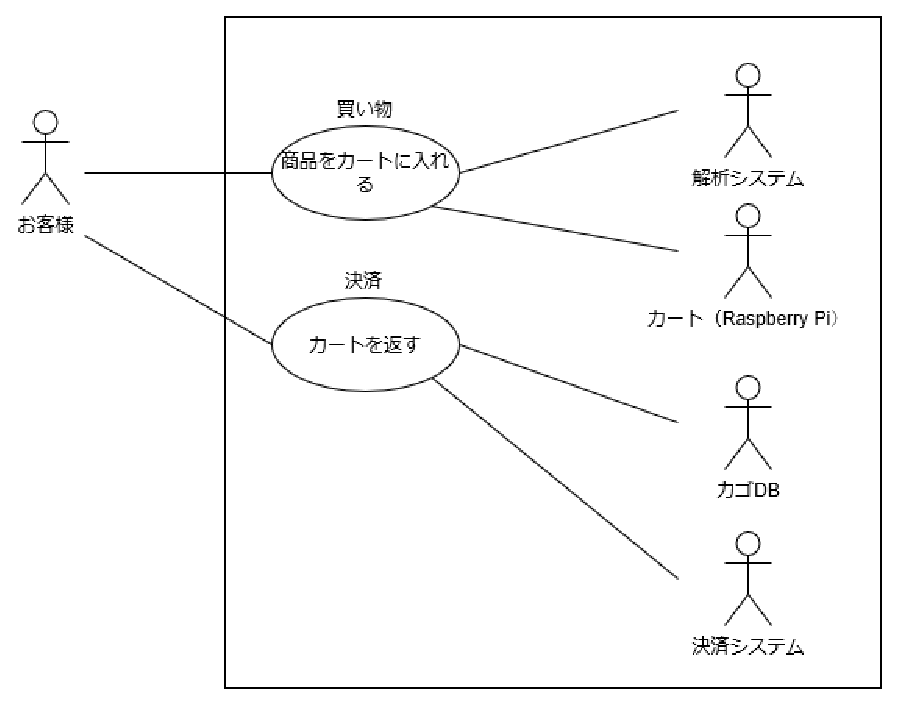
\includegraphics[width=12cm]{./pic/usecase_saishu.eps}
\caption{ユースケース図}
\label{usecase}
\end{figure}

次に、ユースケース図を基に商品識別システムのシナリオを以下の表\ref{scenario}に示す。
\begin{table}[htb]
\begin{center}
\caption{商品識別システムのシナリオ}
\begin{tabular}{|l|c|} \hline
 & シナリオ \\ \hline \hline
買い物 & 商品を置く→バーコード認識→商品DB追加・削除→結果通知 \\
決済 & ユーザが退店する→決済を行う \\ \hline
\end{tabular}
\label{scenario}
\end{center}
\end{table}

%ここおかしい
次に、要求定義を満たすテスト項目を以下の表\ref{./pic/integrated_test}を示す。

\begin{table}[htbp]
\centering
\caption{総合テスト}
\includegraphics[width=15cm]{./pic/integrated_test.eps}
\label{integrated_test}
\end{table}
%第3章2
\section{設計}
\subsection*{基本設計}

ユースケース図の動作を満たすように基本設計を行う。図\ref{usecase}を基に、基本設計を行った。

図\ref{usecase}に示されている項目をもとに、機能別にクラス化を行った。クラスには、カゴ、解析システム、カゴDB、決済システム、商品DBがある。
クラス名カゴの役割は、ユーザがカート内に商品を出し入れする動作全般を行う。クラス名解析システムの役割は、カートに入れられた商品の識別を行う。
カゴDBの役割は、カートに入れられた商品の管理を行うためにある。決済システムの役割は、ユーザが決済を行う際の購入金額の計算および、カゴDBの整理を行う。最後の商品DBの役割は、商品の値段や、商品名、バーコード番号の管理を行うためにある。
\subsection*{詳細設計}
次に、シーケンス図を用いてスマートモビリティレジシステムの手順を説明する。以下の図\ref{sequence}にそって説明する。赤枠で囲っている部分が筆者の実装担当である。
図\ref{sequence}はカート側、サーバ側、Webページ側の3つに大別される。左から右の順に処理を行う。シーケンス図から読み取れるように、ユーザからカートへ商品が渡され、カートで処理を行う。処理が終わると解析システムへ情報が伝達され、解析が始まる。解析結果をカゴDBとカートに送信する。結果はWebページへ反映される。カートではDBの操作は行われない。

図\ref{sequence}において筆者が担当した部分はメッセージの7~10、12~18である。図\ref{sequence}に記述されている筆者が担当したメッセージの具体的な機能と、検証項目(単体テスト項目)について説明していく。

\newpage

\begin{quote}

7.サーバが、RaspberryPiから送信された画像データとフラグを受信する。

8.受信した画像データを画像に変換する。画像を解析してバーコード番号を識別する。

9.受信したフラグを基に、バーコード番号をカゴDBに追加・削除する。

10.サーバからRaspberryPiへ、解析が成功したかどうかの結果(フラグ)を返信する。

12.購入予定商品を管理しているカゴDBを参照し、結果をWebページに表示する。Webページ上では、購入予定商品が、リスト上に表示される。

13.ユーザはWebページで購入予定商品を確認し、購入ボタンを押すことで購入が決定する。

14.決済システムがカゴDBに接続し、決済を行う。

15.商品DBを参照して、ユーザが購入する商品の合計金額を割り出す。なお、商品DBを参照する理由は、カゴDBには購入予定商品のバーコード番号しか管理されているためである。

16.メッセージ15で割り出した合計金額をWebページに表示する。

17.顧客DBに登録されているユーザの所持金から、合計金額を引き決済する。なお、所持金が購入金額より下回っていた場合は、決済は行われない。

18.決済が終了すると、Web画面にユーザの残高が表示される。
\end{quote}

\begin{figure}[htbp]
\centering
\includegraphics[width=15cm]{./pic/sequence_final.eps}
\caption{シーケンス図}
\label{sequence}
\end{figure}

\newpage

次に、筆者が担当した部分が、詳細設計の要件を満たすかの検証を行う。単体テスト項目を作り、検証を行った。

表\ref{server_test}は、メッセージ番号の7,9,10番のRaspberryPiからのデータ通信に関する単体テスト項目である。
\begin{table}[htbp]
\centering
\caption{サーバ単体テスト項目}
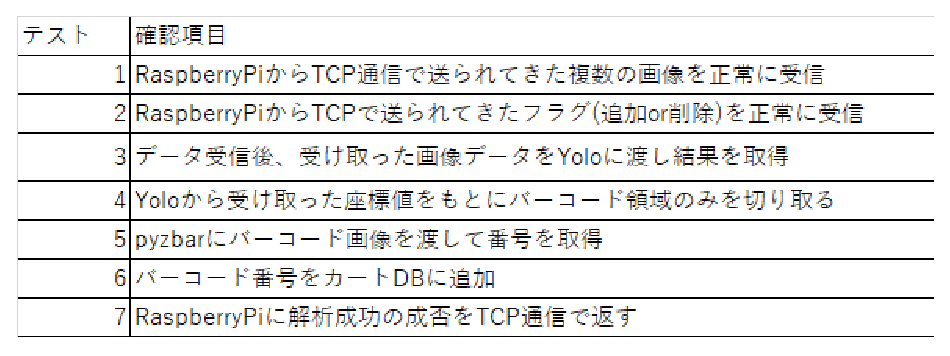
\includegraphics[width=15cm]{./pic/server_test.eps}
\label{server_test}
\end{table}

表\ref{yolo_test}は、メッセージ番号8のバーコード解析についての単体テスト項目である。
\begin{table}[htbp]
\centering
\caption{Yolo単体テスト項目}
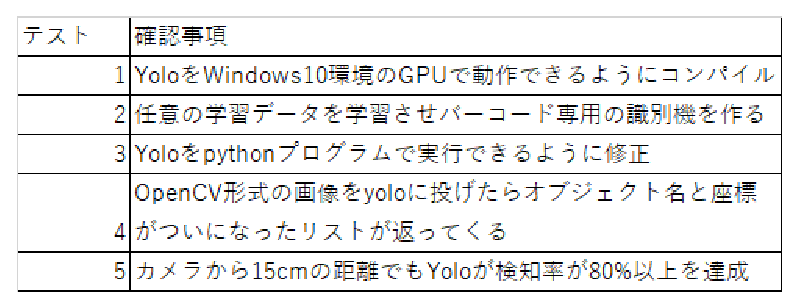
\includegraphics[width=15cm]{./pic/yolo_test.eps}
\label{yolo_test}
\end{table}

\newpage

表\ref{db_test}はメッセージ番号12~18の決済システムに対する単体テスト項目である。
\begin{table}[htbp]
\centering
\caption{決済システム単体テスト項目}
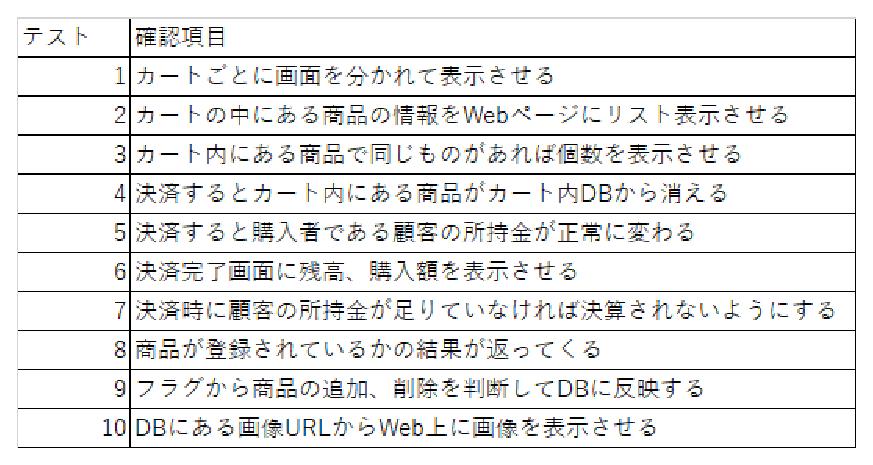
\includegraphics[width=15cm]{./pic/db_test.eps}
\label{db_test}
\end{table}

表\ref{table_test}は、メッセージ番号12の商品DBに対する単体テスト項目である。
\begin{table}[htbp]
\centering
\caption{商品DB単体テスト項目}
\includegraphics[width=15cm]{./pic/table_test.eps}
\label{table_test}
\end{table}


%第4章
\chapter{実装・検証}
%第4章:実験結果・考察

%第4-1章:実装
%手順(実験者のしたこと)


\section{実装}
%第4章:検証
%結果(実験で起こったこと)を書く.客観的に.グラフあればなおよし.


\section{検証}


\subsection{詳細設計の検証}

まず,各種センサが要件を満たすかどうか検証した.

\subsection*{Webカメラ}

対象商品をカメラから100mm,150mm,200mmと離し,バーコードを読み取れるかテストを行った.カゴの高さが240mmかつ,Webカメラの設置場所はカゴの上部90mmのため,150~200mm程度までバーコードが認識できれば構わないとする.

はじめに,WebカメラとしてロジクールC270を使用し,テストを行った.全て画像のピントが合っておらず,バーコードを読み取ることができなかった.より画質が高く,ピントの合いやすいスマートフォンのカメラで撮影した動画でバーコード読み取りを試したところ,100mm,150mm程度まで読み取ることができたため,バーコード読み取りシステムの不具合ではなかったことが判明した.画素数もしくはピントを合わせる機能が問題になっていると仮定した.

次に,Raspberry Pi カメラモジュール V2を使用し,テストを行った.Raspberry Pi カメラモジュール V2については画素数はロジクールC270の約6.6倍の画素数のため,もし画素数に問題があるならば判明すると考えた.Raspberry Pi カメラモジュール V2をテストしたところ,ロジクールC270と同じようにピントが合わず,バーコードを読み取ることができなかった.

画素の問題でないことが判明したため,オートフォーカスモデルのロジクールC615を使用しテストを行った.バーコードの読み取り距離について要求を満たしたため,表\ref{jissou}に最終的な実装環境として,ロジクールウェブカメラC615を記載した.

\subsection*{超音波センサ}

超音波センサが正しく反応しているか,要求を満たしているかテストを行った.要求としてはカゴの横幅360mmなので,360mm以内を10mm程ずつ測ることができるかどうか確認した.超音波センサは正しく反応し,360mm以上の距離を1mmより小さい距離ずつ測ることができ,要求を満たした.

\subsection*{ロードセル}

ロードセルが正しく反応しているか,要求を満たしているかテストを行った.要求として,重量の増減を確認できるか,3kgまでの重量を1g程ずつはかることができるかどうか確認した.ロードセルは正しく反応し,対象商品を1gより小さい値ずつ測ることができた.そのためロードセルは要求を満たした.

\subsection*{LED}

LEDが正しく点灯するかどうか確認した.各LEDを抵抗と共にブレッドボードに設置し,点灯するかテストしたところ,正しく点灯した.


\subsection{単体テスト}

V字モデルに従い,詳細設計を満たしているかどうかを確認する.各実装対象の単体テストの内容を表\ref{tantai}に示す.

\begin{figure}[htbp]
\centering
\caption{単体テスト}
\includegraphics[width = 15cm]{./picture/tantai.eps}
\label{tantai}
\end{figure}

\subsection{結合テスト}


\subsection{総合テスト}


%第5章
\chapter{評価・考察}
%第5章:評価・考察

本章では本システムを評価することにより,今後の課題について述べる.

まず,本システムを評価する.3.1節で設定した,3点の基本の評価軸より評価する.評価したものを書き表\ref{hyouka}に示す.

\begin{table}[htb]
\begin{center}
\caption{システムの評価}
\begin{tabular}{|c|c|} \hline
基本の評価軸 & 評価 \\ \hline \hline
従来のセルフレジよりコストは抑えられるか & 〇 \\
既存の中小店でも導入が容易か & △ \\
従来のセルフレジより簡単な動作で決済まで行えるか & △\\ \hline
\end{tabular}
\label{hyouka}
\end{center}
\end{table}

表\ref{hyouka}を上から順に説明する.従来のセルフレジよりコストは抑えられるかという評価軸について,2.2節で述べた表\ref{taisho}のスーパーマーケットを対象にして確認をする.Raspberry Piの価格は5,700円程度,各種センサと周辺機器の合計価格は3,500円程度のため,カゴにかかる合計価格は約9,200円とする.サーバと周辺機器にかかる価格を約150,000円とする.サーバ1台約150,000円とカゴ90個約828,000円とすると,本システムでかかる価格は約978,000円となり,従来のセルフレジとして2.2節で仮定した登録機1台と精算機7台の合計価格の約5\%程の価格となることが分かった.上記の理由から,従来のセルフレジよりコストを抑えられるとした.

次に,既存の中小店でも導入が容易かという評価軸においては,現段階では容易ではないため△とした.Raspberry Piや各種センサがしっかりと固定されておらず,誰でも導入ができるわけではないことが今後の課題となる.また,保守の点においてもセンサ類等がカゴに設置されるため,保守が難しくなるであろうという問題点もある.しかしながら,これからしっかり固定できるような状況ができれば,既存の買い物カゴに設置できる規模感であるため可能性がある.また,保守についても,抑えられたコストから少数の人員を割くことができ,解決ができるだろう.

次に,従来のセルフレジより簡単な動作で決済まで行えるかという評価軸においては,現時点では,商品のバーコードを読み取らせるために商品を回転させ,バーコードリーダを操作するような動作は必要はないが,バーコードをWebカメラに向けて台に置く必要があるため△とした.また,精度についても各センサの誤作動もあるため,完全であるとは言い切れない.簡単な動作で決済まで行えるかどうかについては問題点となる.しかしながら,バーコードがWebカメラに向けて置かれなかった場合についても,YOLOの開発が進めば商品のジャンルを判定できる可能性がある.また,ロードセルより重量のデータを得ることができるため,重量データと掛け合わせて商品を確定することができる可能性もある.画像識別の技術開発が進めば,バーコード情報だけでなく商品の情報を読み取ることができるという利点を持つWebカメラをモビリティショッピング端末に用いているため拡張性があるといえる.よって今後解決や開発が進めば可用かつ拡張性のあるシステムであると考えた.


%%評価・考察


\section{評価}
%%第5章:考察
%考察(起こったことに対する理由付けや解釈)を書く.主観的でよい.


\section{考察}



%第6章
\chapter{あとがき}
%あとがき,結論
%5-1研究の成果(考えたこと,わかったこと)を書く(結論表),5-2成果の価値(学術的価値や実用的価値)を書く(先発性・明晰性・普遍性・可用性),5-3今後の課題(成果の限界とその克服のための戦略)を書く(アイデアの平凡さ・あいまいさ・狭さ・非実用性を検討

本論文ではセンシング技術を用いたモビリティショッピング端末の開発を行った.V字モデルに従い,要求分析,基本設計,詳細設計を行い,グループで役割分担をし開発を行った.システム全体の設計としては,UMLを用いて方針を固めた.実装においては,優先度の高い機能を実装し,それぞれの単体テスト,結合テスト,総合テストを通して動作を確認し,評価を行った.検証を行う際,問題があった場合はそれぞれの設計に戻り,再度検証を行った.検証を行ったシステムを評価軸に沿って評価し,今後の課題について考察した.本システムは小規模店舗,中規模店舗を対象とし,コストを抑えたシステムとして先発性がある.本システムの開発が進めば,小規模店舗,中規模店舗での人手不足問題が解消される.本研究により本システムは今後拡張性があり,低コストで運用ができる可能性を持つシステムであることを確認した.
%--ここまで本文--


%謝辞
\newpage
\addcontentsline{toc}{chapter}{\protect\numberline{謝辞}{}}
\chapter*{謝辞}
%--ここから謝辞--
本研究を進めるにあたり,懇篤な御指導,御鞭撻を賜わりました本学高橋寛教授に深く御礼申し上げます.

本論文の作成に関し,詳細なるご検討,貴重な御教示を頂きました本学樋上喜信准教授ならびに王森レイ講師に深く御礼申し上げます.

また,審査頂いた本学高橋寛教授ならびに遠藤慶一准教授,木下浩二講師に深く御礼申し上げます.

最後に,多大な御協力と貴重な御助言を頂いた本学工学部情報工学科情報システム工学講座高橋研究室の諸氏に厚く御礼申し上げます.

%--ここまで謝辞--

%参考文献
\begin{thebibliography}{99}
%ここから参考文献

%--例--
\bibitem{population}
平成28年版 情報通信白書|人口減少社会の到来,総務省,https://www.soumu.go.jp/johotsusintokei/whitepaper/ja/h28/html/nc111110.html,2016-07


\bibitem{super}
一般社団法人 全国スーパーマーケット協会,年次統計調査 2019年調査,http://www.super.or.jp/wp-content/uploads/2019/10/2019nenji-tokei.pdf,2019-10


\bibitem{uml}
株式会社 オージス総研,かんたんUML[増補改訂版],株式会社 翔泳社,2003


\bibitem{kumikomi}
阪田史郎,高田広章,組込みシステム,株式会社 オーム社,2006


\bibitem{soft}
小泉寿男,辻 秀一,吉田 幸二,中島 毅,ソフトウェア開発,株式会社 オーム社,2003


\bibitem{reji}
レジチョイス編集部,価格・製品特徴比較,https://rejichoice.jp/semi-self-regi/,2020-01-15

%ここまで参考文献

\end{thebibliography}
\end{document}
